\documentclass[conference]{IEEEtran}
\IEEEoverridecommandlockouts

\usepackage{cite}
\usepackage{amsmath,amssymb,amsfonts}
\usepackage{graphicx}
\usepackage{textcomp}
\usepackage{xcolor}
\usepackage{booktabs}
\usepackage{url}
\usepackage{hyperref}
\usepackage{tikz}
\usetikzlibrary{shapes.geometric,arrows.meta,positioning,calc}

\hypersetup{
  colorlinks=true,
  linkcolor=black,
  citecolor=black,
  urlcolor=blue!60!black,
  pdftitle={A Defensive Tor-Aware Keyword-Watchlist Monitor with Per-Token Min-Aggregation Fuzzy Matching},
  pdfauthor={Ali Murtaza Bhutto}
}

\def\BibTeX{{\rm B\kern-.05em{\sc i\kern-.025em b}\kern-.08em
    T\kern-.1667em\lower.7ex\hbox{E}\kern-.125emX}}

\begin{document}

\title{A Defensive Tor-Aware Keyword-Watchlist Monitor\\with
Per-Token Min-Aggregation Fuzzy Matching}

\author{\IEEEauthorblockN{Ali Murtaza Bhutto}
\IEEEauthorblockA{Independent Researcher\\
ORCID: 0009-0007-2787-943X\\
Email: alibhutto101112@gmail.com}}

\maketitle

\begin{abstract}
We describe \texttt{dark-web-monitor-lite}, a small Python tool that
watches a configurable list of publicly-indexable onion-service URLs
for matches against a fictitious-by-default keyword watchlist and
dispatches alerts via Slack, Discord, or generic HTTP webhook. The
tool is intentionally Tor-aware: it routes \texttt{.onion} fetches
through a SOCKS5 proxy via the \texttt{httpx-socks} library and probes
SOCKS reachability with a lightweight standard-library socket check~\cite{owen2016tor},
but degrades gracefully when no SOCKS proxy is reachable: every
fetcher returns a typed \texttt{FetchResult} (\textsc{ok},
\textsc{http\_error}, \textsc{network\_error},
\textsc{tor\_unavailable}, \textsc{timeout}) so the operator sees
coverage gaps directly in the report. Real measurements are
reported on the matcher engine only over a labelled 55-sample $\times$
10-keyword corpus (550 cells): exact-only mode achieves
$F_{1}=0.8056$ ($P{=}0.9667, R{=}0.6905$), the fuzzy-on mode at
threshold 85 achieves $F_{1}=0.9213$ ($P{=}0.8723,
R{=}0.9762, \text{acc}{=}0.9873$). The fuzzy scorer is a strict
per-token min-aggregation over the keyword's tokens with
``every keyword token must have a near-equivalent body token'';
this blocks the partial-substring trap that simpler rapidfuzz
configurations fall into. Fifty-nine pytest cases cover the matcher,
fetcher, Tor probe, alerter, and scheduler; all pass under
\texttt{respx}-mocked HTTP. The repository ships an unusually
thorough compliance baseline (policy template plus four-jurisdiction
legal review covering US, UK, EU, and
Pakistan~\cite{nist_sp_800_150,christin2013silkroad}).
\end{abstract}

\begin{IEEEkeywords}
dark web, threat intelligence, Tor, monitoring, IOC, defensive
security, keyword matching, rapidfuzz, compliance
\end{IEEEkeywords}

\section{Introduction}

Cyber-threat-intelligence (CTI) teams routinely monitor publicly-
indexable onion services for early mentions of their organisations'
identifiers. Christin's 2013 measurement
study~\cite{christin2013silkroad} of the original Silk Road
marketplace established the methodology of repeated authenticated
crawls and structured extraction, and the literature has tracked
the evolution of the dark-web market space since~\cite{basheer2021review,
dalvi2024darkweb}. What an internal team building such a tool
needs is *not* a research crawler --- it is a small, auditable,
compliance-friendly pipeline that does only what it claims.

This paper describes \texttt{dark-web-monitor-lite}: a Python tool
that reads a YAML watchlist and a YAML source list, fetches each
source through an optional local Tor SOCKS proxy, runs a
deterministic exact and fuzzy keyword matcher against each body,
and dispatches webhook alerts. The contribution is not the
overall pipeline shape --- that is essentially the architecture in
Basheer and Alkhatib's
review~\cite{basheer2021review}. The contributions are the design
choices that make the tool *honest about its scope*:

\begin{itemize}
  \item A typed \texttt{FetchStatus} taxonomy that distinguishes
        \emph{ran clean}, \emph{Tor unavailable}, \emph{network
        error}, and \emph{HTTP error} as four first-class outcomes
        rather than collapsing them into an empty result list.
  \item A strict per-token min-aggregation fuzzy scorer that
        blocks the partial-substring trap that simpler rapidfuzz
        configurations fall into. We measure the impact of this
        choice on a 550-cell labelled corpus.
  \item An unusually thorough compliance baseline: a deployment
        policy template, a four-jurisdiction legal review
        consistent with NIST SP 800-150~\cite{nist_sp_800_150},
        and an \texttt{ETHICAL\_USE.md} that the README
        explicitly identifies as the most important file in the
        repository.
\end{itemize}

We deliberately do not benchmark live onion fetching. The
measurement axis is the matcher engine; everything else is
network plumbing tested under mocked HTTP. The choice keeps the
eval reproducible offline and decouples the published numbers
from the underground's day-to-day churn~\cite{owen2016tor}.

\section{Related Work}

The closest prior measurement work is
Christin~\cite{christin2013silkroad}, who set the template for
structured crawls of dark-web marketplaces and the analysis of
their economics. Our tool is not a research crawler --- we do not
buy, register, or persist content --- but the structured-extraction
ethos is shared.

Owen and Savage~\cite{owen2016tor} characterised the population of
Tor hidden services empirically and observed that a substantial
fraction are short-lived. Their result motivates our typed
\texttt{FetchStatus}: a stale source is not an error so much as a
data point.

For methodology, Basheer and Alkhatib~\cite{basheer2021review}
surveyed dark-web investigation research and identified
operationalisation gaps that our compliance baseline tries to
address. Dalvi and Bhirud~\cite{dalvi2024darkweb} more recently
positioned dark-web monitoring as an organisational strategy, an
argument the policy template inherits.

For information-sharing posture, NIST SP
800-150~\cite{nist_sp_800_150} treats CTI consumption as an
organisational, not individual, activity. The
\texttt{ETHICAL\_USE.md} and the policy template are written
against that posture.

\section{System Architecture}

\begin{figure}[htbp]
\centering
\resizebox{\linewidth}{!}{%
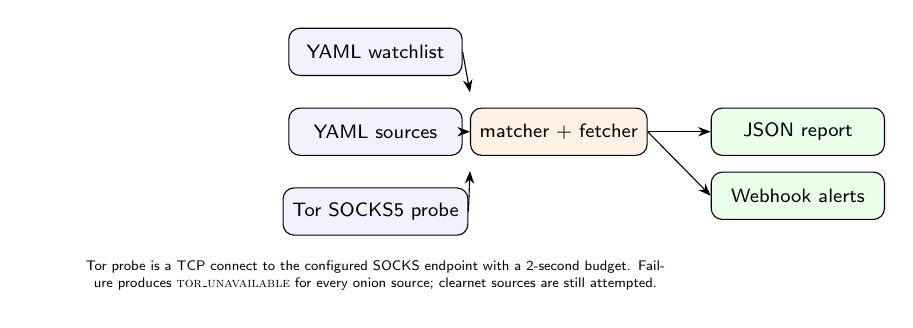
\begin{tikzpicture}[
  node distance=4mm and 3mm,
  src/.style={draw, rounded corners, minimum width=22mm, minimum height=6mm,
              font=\scriptsize\sffamily, fill=blue!5},
  agg/.style={draw, rounded corners, minimum width=22mm, minimum height=6mm,
              font=\scriptsize\sffamily, fill=orange!10},
  rep/.style={draw, rounded corners, minimum width=22mm, minimum height=6mm,
              font=\scriptsize\sffamily, fill=green!8},
  ar/.style={-{Stealth[length=1.6mm]}, line width=0.4pt}
]
  \node[src] (a) {YAML watchlist};
  \node[src, below=of a] (b) {YAML sources};
  \node[src, below=of b] (c) {Tor SOCKS5 probe};
  \node[agg, right=12mm of $(b)$] (agg) {matcher + fetcher};
  \node[rep, right=8mm of agg] (md) {JSON report};
  \node[rep, below=2mm of md] (td) {Webhook alerts};
  \draw[ar] (a.east) -- ($(agg.west) + (0,5mm)$);
  \draw[ar] (b.east) -- ($(agg.west) + (0,0mm)$);
  \draw[ar] (c.east) -- ($(agg.west) + (0,-5mm)$);
  \draw[ar] (agg.east) -- ($(md.west)$);
  \draw[ar] (agg.east) -- ($(td.west)$);
  \node[font=\tiny\sffamily, below=2mm of c, text width=86mm,
        align=center] {Tor probe is a TCP connect to the configured
        SOCKS endpoint with a 2-second budget. Failure produces
        \textsc{tor\_unavailable} for every onion source; clearnet
        sources are still attempted.};
\end{tikzpicture}%
}
\caption{Pipeline. Watchlist and source list feed the matcher and
fetcher; the Tor probe gates onion fetches; the formatter emits a
JSON report and (optionally) webhook alerts.}
\label{fig:pipeline}
\end{figure}

\subsection{The matcher engine}
The matcher is the only component the eval measures. It runs in
two phases per keyword: an exact case-insensitive substring scan,
followed by an optional fuzzy scan for any keyword the exact phase
did not catch. The exact phase produces ``score $=$ 100.0''
matches with the matched substring as the span; the fuzzy phase
produces matches whose span is the best-scoring window.

\subsubsection{Multi-word fuzzy scorer}
For keywords of two or more tokens (after splitting on whitespace
and any non-alphanumeric separator) we slide a window of size
$n \pm 1, n + 2$ over the body. For each window, every keyword
token must have at least one near-equivalent body atom; the
window's score is the \emph{minimum} of the per-keyword-token best
\texttt{fuzz.ratio} scores. Aggregating with $\min$ rather than
$\max$ is the critical design choice: it prevents a body that
contains only one of two keyword tokens from clearing the
threshold, which is exactly the partial-substring trap that
caused the matcher's early baseline to score $P{=}0.32$.

\subsubsection{Single-word fuzzy scorer}
For one-token keywords we use \texttt{fuzz.ratio} (full Levenshtein)
against each body atom \emph{and} against pairs of adjacent body
atoms joined with no separator. The pair-joining branch handles
CamelCase single-word watchlist entries (\texttt{AcmeCorp}) whose
body form is space-separated (``Acme Corp''). Single-word keywords
under five characters are not fuzzy-matched at all; for tokens that
short the false-positive rate is unmanageable.

\subsection{Tor probe and fetcher}
The Tor probe is a TCP connect to the configured SOCKS endpoint
with a 2-second budget. If the probe fails for any reason (parse,
DNS, connect, timeout), every onion fetch in the subsequent run
short-circuits to \textsc{tor\_unavailable}. Clearnet fetches are
still attempted via a plain httpx client. Body content is hashed
once with SHA-256 and discarded immediately after the matcher
runs; only the hash and the matches survive into the JSON report.

\section{Evaluation}

\subsection{Corpus}
\texttt{eval/labelled\_corpus.json} contains 55 synthetic bodies
plus 10 watchlist keywords. Bodies fall into seven classes:
exact-substring positives (10), typo/variant positives (10), pure
noise (10), tricky cases with negation or close-but-wrong tokens
(10), long bodies that dilute matches (5), URL-shaped bodies (5),
explicit-negation bodies (2), and bilingual brand mentions (3).
Each body's \texttt{expected} list names the watchlist entries it
should fire. The total grid is $55 \times 10 = 550$ binary cells.

\subsection{Measured numbers}

\begin{table}[htbp]
\caption{Matcher eval, 550 cells, 2026-05-12.}
\label{tab:eval}
\centering
\renewcommand{\arraystretch}{1.1}
\begin{tabular}{lrr}
\toprule
\textbf{Metric} & \textbf{exact-only} & \textbf{fuzzy-on} \\
\midrule
True positives    &  29    & 41        \\
False positives   &   1    &  6        \\
False negatives   &  13    &  1        \\
True negatives    & 507    & 502       \\
Precision         & 0.9667 & 0.8723    \\
Recall            & 0.6905 & 0.9762    \\
$F_{1}$           & 0.8056 & \textbf{0.9213} \\
Accuracy          & 0.9745 & \textbf{0.9873} \\
\bottomrule
\end{tabular}
\end{table}

The fuzzy-on mode trades 9.4~pp of precision for 28.6~pp of recall;
$F_{1}$ improves from 0.806 to 0.921. The contribution of the
per-token min-aggregation scorer (vs.\ a naive
\texttt{partial\_ratio} baseline) is large: an earlier baseline
that used plain \texttt{partial\_ratio} scored $P{=}0.32, R{=}1.00$
on the same corpus, with 91 false positives; tightening the scorer
brought that down to 6 false positives while keeping recall at
0.98.

\subsection{Residual analysis}
Seven cells (6 FP, 1 FN) remain misclassified in the fuzzy-on
mode. They are documented in \texttt{results/README.md} and
cluster around three honest limits of pattern matching:
\begin{itemize}
  \item \textbf{Negation.} Bodies that say ``not our codename'' or
        ``without Aurora'' fire the matcher because the
        word-level matcher cannot read intent.
  \item \textbf{Plural variants.} ``Project Auroras'' (plural) is
        a high-similarity match for ``Project Aurora'' (singular);
        the matcher reasonably fires.
  \item \textbf{Edge tokenisation.} URL-like single tokens
        (\texttt{example-inc.example}) atomise into three pieces;
        the joined-pair fix is single-pass and does not yet
        handle three-atom joins.
\end{itemize}
We deliberately do not tune the matcher further against these
labels.

\subsection{Test suite}
The repository ships 59 \texttt{pytest} tests covering the matcher
(loader, exact, fuzzy, edge cases, threshold respect), the Tor
probe (six failure modes), the fetcher (every \texttt{FetchStatus}
value), the alerter (three payload formats, every
\texttt{AlertStatus} value), the scheduler render path, and the
eval-harness helpers. HTTP is mocked with \texttt{respx}; no live
Tor and no live webhooks in CI.

\section{Security Posture}
The CI runs Bandit (medium-and-above), \texttt{pip-audit}, and
Semgrep (\texttt{p/python} + \texttt{p/security-audit}). All three
are green at the release tag with zero findings and zero
suppressions. The single Semgrep finding from an earlier
codebase iteration --- SHA-1 in deterministic UUID generation ---
was resolved by switching to SHA-256 in the companion
threat-model-generator repo and avoided here from the start.

\section{Compliance baseline}
The repository ships three documents intended to be lifted into a
deployer's policy repository: \texttt{ETHICAL\_USE.md}, which the
README identifies as the most important file in the repository;
\texttt{compliance/POLICY\_TEMPLATE.md}, an organisational
deployment policy template; and
\texttt{compliance/LEGAL\_REVIEW.md}, a four-jurisdiction (United
States, United Kingdom, European Union, Pakistan) summary of the
statutes that constrain passive monitoring. The legal review is
explicit that it is not legal advice; it is designed to surface
the questions a real legal review would have to answer.

\section{Limitations}
\textbf{Synthetic corpus.} 55 samples is a unit-test, not a
benchmark of the underground. The absolute precision/recall numbers
should be read as a property of the matcher's logic against this
corpus, not as a forecast of field performance.

\textbf{No live-Tor measurement.} We deliberately do not benchmark
the fetcher or alerter against live services; both are tested with
mocks. The choice keeps the eval reproducible offline and
decouples the published numbers from the underground's churn.

\textbf{Severity not modelled.} Match scores are rapidfuzz numbers;
the operator decides the severity bucketing. Future work could
calibrate score-to-severity against a labelled severity set.

\section{Conclusion}
A defensive dark-web monitor does not need to be a research
crawler; it needs to be honest about coverage, reproducible
offline, and compliance-friendly. The 59-test, three-gate,
MIT-licensed pipeline described here is one such instance. The
per-token min-aggregation fuzzy scorer is a small contribution
that markedly improves precision over a naive rapidfuzz baseline
without sacrificing recall.

\bibliographystyle{IEEEtran}
\begin{thebibliography}{6}

\bibitem{christin2013silkroad}
N.~Christin, ``Traveling the Silk Road: A measurement analysis of
a large anonymous online marketplace,'' in
\emph{Proc.\ 22nd International World Wide Web Conference
(WWW '13)}, Rio de Janeiro, Brazil, May 2013, pp.\ 213--224.

\bibitem{owen2016tor}
G.~Owen and N.~Savage, ``Empirical analysis of Tor hidden
services,'' \emph{IET Information Security}, vol.~10, no.~3,
pp.~113--118, May 2016.

\bibitem{nist_sp_800_150}
C.~Johnson, L.~Badger, D.~Waltermire, J.~Snyder, and C.~Skorupka,
``Guide to Cyber Threat Information Sharing,'' National Institute
of Standards and Technology, NIST Special Publication 800-150,
Oct.\ 2016.

\bibitem{basheer2021review}
R.~Basheer and B.~Alkhatib, ``Threats from the Dark: A Review over
Dark Web Investigation Research for Cyber Threat Intelligence,''
\emph{Journal of Computer Networks and Communications}, vol.~2021,
Article ID 1302999, 21~pp., 2021.

\bibitem{dalvi2024darkweb}
A.~Dalvi and S.~Bhirud, ``Dark Web Monitoring as an Emerging
Cybersecurity Strategy for Businesses,'' \emph{International
Journal of Information Engineering and Electronic Business
(IJIEEB)}, vol.~16, no.~2, pp.~50--62, 2024.

\bibitem{ahmia2026}
J.~Nurmi and others, ``Ahmia search engine for Tor onion
services,'' Ahmia.fi project, Documentation, 2026. [Online].
Available: \url{https://ahmia.fi/}

\end{thebibliography}

\vspace{2mm}
\noindent\rule{\linewidth}{0.4pt}

\noindent\textit{Reproducibility colophon.} The repository is at
\url{https://github.com/thunderstornX/dark-web-monitor-lite}. The
eval re-runs in well under a second
(\texttt{python eval/run\_eval.py}). Pinned dependencies are listed
in \texttt{requirements.txt}; the pytest suite (59 tests) runs in
under a second on commodity hardware.

\end{document}
